%\documentclass[12pt]{article}
\documentclass[12pt]{revtex4}
%\documentclass[draft,12pt]{article}
\usepackage{amsmath}
\usepackage{amsfonts}
\usepackage{amsbsy}
\usepackage{lscape} 
\usepackage{color}
\usepackage{graphicx,epsfig}
\usepackage[english]{babel}
\usepackage{latexsym}
\usepackage{amssymb}
%\usepackage{palatino}
%\usepackage{chancery}
%\usepackage{newcent}
%\usepackage{charter}
%\usepackage{zapfchan}
%\usepackage{bookman}
%\usepackage{sparticles}        %Package for displaying sparticle names. 
%\usepackage{feynmf}            %Package for feynman diagrams. 

\newcommand{\beq}{\begin{equation}}
\newcommand{\eeq}{\end{equation}}

\newcommand{\eq}{{\rm eq}}
\newcommand{\lgr}{\left\lgroup}
\newcommand{\rgr}{\right\rgroup}
\newcommand{\Mpl}{M_{\rm Pl}}
\newcommand{\Tfr}{T_{\rm fr}}
\newcommand{\Tsph}{T_{\rm sph}}
\newcommand{\Gsph}{\Gamma_{\rm sph}}
\newcommand{\Eray}{E_{\rm ray}}
\newcommand{\meff}{m^{\rm eff}_\nu}

\newcommand{\p}{\partial}
\newcommand{\mc}[1]{\mathcal{#1}}
\newcommand{\md}{\mathcal{D}}
\newcommand{\wt}{\widetilde}
\newcommand{\ov}{\overline}
\newcommand{\suc}{{\rm SU}_{\rm C}(3)}
\newcommand{\sul}{{\rm SU}_{\rm L}(2)}
\newcommand{\ue}{{\rm U}(1)}
\newcommand{\GeV}{{\rm GeV}}
\newcommand{\eV}{{\rm eV}}
%\newcommand{\su3}{{\rm SU}_{\rm C}(3)}

%%%%%%%%%%%%%%%%%%%%%%%%%%%%%%%%%%%%%%%
%  Slash character...
\def\slashed#1{\setbox0=\hbox{$#1$}             % set a box for #1
   \dimen0=\wd0                                 % and get its size
   \setbox1=\hbox{/} \dimen1=\wd1               % get size of /
   \ifdim\dimen0>\dimen1                        % #1 is bigger
      \rlap{\hbox to \dimen0{\hfil/\hfil}}      % so center / in box
      #1                                        % and print #1
   \else                                        % / is bigger
      \rlap{\hbox to \dimen1{\hfil$#1$\hfil}}   % so center #1
      /                                         % and print /
   \fi}                                        %

%%EXAMPLE:  $\slashed{E}$ or $\slashed{E}_{t}$


\begin{document}

%%
%% The title page
%% 
\begin{titlepage}
\renewcommand{\thefootnote}{\fnsymbol{footnote}}

\setcounter{page}{1}

\vspace*{0.2in}

\begin{center}

\hspace*{-0.6cm}\parbox{17.5cm}{\Large \bf \begin{center}
$CPT$-odd Leptogenesis\end{center}}

\vspace*{0.5cm}
\normalsize


{\bf Pavel Bolokhov$^{\,(a,b)}$ and Maxim Pospelov$^{\,(a,c)}$ }



\smallskip
\medskip

$^{\,(a)}${\it Department of Physics and Astronomy, University of Victoria, \\
     Victoria, BC, V8P 1A1 Canada} \\
$^{\,(b)}${\it Theoretical Physics Department, St.Petersburg State University, Ulyanovskaya 1,
        Peterhof, St.Petersburg, 198504, Russia}\\
$^{\,(c)}${\it Perimeter Institute for Theoretical Physics, Waterloo,
ON, N2J 2W9, Canada}

\smallskip
\end{center}
\vskip0.2in


\centerline{\large\bf Abstract}

We calculate the baryon asymmetry of the Universe resulting from 
higher-dimensional Lorentz-noninvariant $CPT$-odd operators and heavy 
Majorana neutrinos. Unlike the standard $CP$-odd scenario, the $CPT$-odd version of
leptogenesis requires only one heavy Majorana neutrino, and the size of the 
resulting asymmetry is directly related to the observable neutrino masses. 
Confronting the range for the  $CPT$-violating dimension five operators
capable of producing observed baryon asymmetry, $10^{-5}M_{\rm Pl}^{-1}$, 
with the direct constraints from low-energy tests of Lorentz invariance and the high-energy
astrophysics bounds, we conclude that current data strongly disfavor the $CPT$-odd
mechanism.  


\vfil
\leftline{August 2006}

\end{titlepage}


%%%%%%%%%%%%%%%%%%%%%%%%%%%%%%%%%%%%%%%%%%%%%%%%%%%%%%%%%%%%%%%%%%%%%%
%%%%%%%%%%%%%%%%%%%%%%%%%%%%%%%%%%%%%%%%%%%%%%%%%%%%%%%%%%%%%%%%%%%%%%
%
%                            INTRODUCTION
%
%%%%%%%%%%%%%%%%%%%%%%%%%%%%%%%%%%%%%%%%%%%%%%%%%%%%%%%%%%%%%%%%%%%%%%
%%%%%%%%%%%%%%%%%%%%%%%%%%%%%%%%%%%%%%%%%%%%%%%%%%%%%%%%%%%%%%%%%%%%%%
\section{Introduction}
\label{intro}

%---	Sakharov's conditions
%
%---	reference to Kostelecky's paper
%
%---	Features of CPT-odd leptogenesis, including equilibrium distribution
%
%---	Leptogenesis epoch, sphaleron epoch
%
%---	unnecessity to having more than one heavy neutrinos
%
%---	Declare analysis of Boltzmann equations for operators of 
%	dimension five, and general arguments for higher-dimensional
%	operator
%
%---	Heavy neutrino interaction, effective lagrangian

Since the seminal paper by Sakharov \cite{Sakharov:1967dj}, it is well known that the 
baryon asymmetry of the Universe (BAU) can be generated dynamically, through the 
combination of baryon number violating processes, $C$ and $CP$ violation, and the 
departure from thermal equilibrium. It turns out that the Stadard Model (SM) has all necessary  
ingredients for this to happen. Notably, the $B+L$ number is violated by the 
high-temperature sphaleron process \cite{Klinkhamer:1984di},\cite{Kuzmin:1985mm}. However, the 
existing amount of $CP$-violation combined with tight constraints on the Higgs sector,
prevent efficient baryogenesis in the SM. Thus, BAU presents a formidable hint of physics 
beyond SM, and motivates new experimental searches for the extended 
electroweak sector and new sources of $CP$ violation. 


	It is also known for some time that $CPT$-odd perturbations of a theory can effectively
	replace two Sakharov's conditions for baryogenesis: violation of $CP$
	invariance and the deviation from thermal equilibrium \cite{Dolgov:1981hv}.
	Indeed, a $CPT$-odd shift in the "mass" of a SM fermion (e.g. top quark \cite{Dolgov:1991fr}), 
    $\Delta m_{CPT}$ 
    would serve as an effective chemical shift between baryons and antibaryons above the 
    scale of the electroweak phase transition. 
    It is easy to see that $\Delta m_{CPT}/m_t\sim O(10^{-6})$ effect for top quark would be required to generate the 
    observed asymmetry  \cite{Dolgov:1991fr}. Unfortunately, at the level of the Lagrangian 
    is impossible to define a consistent 
    "$CPT$-odd mass" without breaking the Lorentz invariance.  $CPT$-odd mass would have to be identified 
with dimension 3 Lorentz-noninvariant operators \cite{Kost1}. Given the strength of
	constraints on lower-dimensional CPT/Lorentz noninvariant operators \cite{Colladay:1998fq}, one 
	has to conclude that they cannot be a source of the observed baryon asymmetry. 

    
%To see the "equivalence" of $CP$-violation combined with non-equilibrium evolution and $CPT$-violation, 
%5one can consider an example of the CP-odd operator composed from a scalar field coupled to the {\em e.g.} pseudoscalar combination 
%of the 

    
	
	%The main reason for this is that baryon asymmetry is present in the
	%equilibrium plasma due to the CPT-odd shifts of the dispersion relations
	%for baryons.
	%That means that, as long as one has a CPT-odd model with baryons in equilibrium,
	%a non-zero BAU will be generated.
%	In some sense the problem of BAU becomes somewhat trivial: one only has
%	to add proper perturbations to the theory.
	
	
	
	The problem of $CPT$-odd baryogenesis was readdressed in \cite{Bertolami:1996cq}
and recently in \cite{Carroll:2005dj}, where higher-dimensional $CPT$-odd operators 
were suggested as a source for baryon asymmetry. Suppose that a dimension five operator that 
shifts the dispersion relations of baryons relative to antibaryons is added on top of the SM. 
Let us furhter assume that initial value for $B-L$ is zero.
Then in the temperature range from $10^{10}$ to $10^2$ GeV where the sphaleron processes are in thermal 
equilibrium, the resulting baryon asymmetry will be determined by the amount of $CPT$ violation in the 
theory. If $CPT$-violating interactions are given by dimension five interaction parametrized by $\eta$, inverse of
the energy scale of $CPT$ violation, the resulting baryon 
asymetry at the sphaleron freeze-out ($T\sim M_W$) will be given by 
\begin{equation}
\label{baryo}
	Y_B ~~=~~ \frac{\Delta B}{S} ~~\sim~~ \eta\, T_{min}~ \sim \eta\, M_W~,
\end{equation}
	where $ S $ is the entropy. It is clear then that $\eta \sim 10^{-12}$ $GeV^{-1}$ will 
	be required to produce an observable asymmetry \cite{Carroll:2005dj}. 
Given the fact that both low-energy data and 
	astrophysical constraints limit a typical $\eta$ better than the inverse Planck scale,
	such scenario is completely ruled out modulo some extreme fine-tuning. 


%	Another problem is that there must have been B-violating processes which kept
%	the plasma in equilibrium.
%	Since such processes do not exist in the Standard Model, one has to introduce
%	new degrees of freedom and interactions.
%	Typically, however, e.g. in the case of GUTs, the pre-generated baryon asymmetry
%	will be matched with the pre-generated lepton asymmetry, and therefore both
%	of them will be washed out by sphalerons, which poses another problem.

%	In general, a successful baryogenesis needs production of $ B - L $, but it does
%	not necessarily have to be a pure baryon number.

    In this paper we explore the idea of the $CPT$-odd leptogenesis that is capable of 
    enhancing the estimate (\ref{baryo}) by many orders of magnitude. 
    The main feature of any leptogenesis scenario is the use of the lepton number non-conservation 
    at high temperatures that results in a nonvanishing $ B - L $ 
    number, that is preserved by sphaleron processes \cite{Fukugita:1986hr}. 
	%At energies $ \Tsph ~\sim~ 10^{12}~\GeV $ sphaleron processes become fast and 
	%diffuse $ B - L $ equally between leptons and baryons. 
	One of the advantages of leptogenesis is that the most natural way of mediating
the lepton-violating processes is through
	heavy majorana neutrinos, which also supplies mass to the light neutrinos
	via the see-saw mechanism. 
	Heavy right-handed neutrinos mediate lepton number violating processes, and thus keep
	lepton number violating processes in equilibrium 
until the temperature decreases to the point where the Hubble rate begins to dominate
over the lepton-violation rate.
	In the assumption that Yukawa couplings are on the order $O(1)$, this moment in the Universe's 
	history can be determined as 
\[
	\Gamma_L ~~\propto~~ \frac{T^3}{M_R^2} ~~\sim~~ H_r ~~\propto~~ \frac{T^2}{\Mpl},
\]
	which gives an estimate for the temperature of the freeze-out for the $B-L$ number:
\[
	T_R ~~\propto~~ \frac{M_R^2}{\Mpl}~.
\]
	Therefore, in the scenarios of CPT-odd leptogenesis, one obtains the asymmetry
	which freezes out at $ T = T_R $ rather than at $ T = M_W $:
\[
	Y_{L(B)} ~~\sim~~ \eta_L\, \frac{M_R^2}{\Mpl}~.
\]
	Obviously, for 	$ M_R \sim 10^{15}~\GeV $ one gets a great enhancement 
	by $ T_R/M_W \sim 10^{9}$ over the $CPT$ baryogenesis scenarios where 
$B-L$ is zero \eqref{baryo}.

%	One, however, still has the problem of B-nonconservation: to keep the plasma
%	in equilibrium one needs B-violating processes, which do not exist in the
%	Standard Model.
%	There are well-known solutions to this problem which extend slightly beyond
%	the Standard Model, for example, into GUTs, where the baryon number is not
%	conserved.
%such that B-violating processes 
%	can proceed.
%	It is easy then to compute the equilibrium number density of baryons.

    
    The purpose of this paper is to explore the $CPT$-odd leptogenesis scenario, 
    determine the required strength of the $CPT$-violating operators, and confront it with the 
    existing laboratory and astrophysics constraints. 
	%Despite some CPT-odd baryogenesis has already been covered in the literature 
%\cite{Carroll:2005dj,Dolgov:1981hv,Dolgov:1991fr,Cohen:1987vi,Bertolami:1996cq},
%	[Carroll, Kostelecky, Zeldovich, Dolgov, Kaplan], 
	%and indicated as a capable mechanism for baryon number generation.
	%However, one of the important goals is to connect the observed BAU with the existing 
	%constraints on LV interactions.
%, which was ?partly? done in [Kostelecky]. 
%	It turns out that to present a detailed numerical prediction for baryon asymmetry, 
%	However, to present a more detailed numerical prediction for baryon asymmetry, 
%	one needs to take into consideration the kinetic equations for baryon number density,
%	as baryon-violating processes not always were in equilibrium.
	%In the case of leptogenesis, 
	%it turns out that to present a numerical prediction for the asymmetry, 
	%one needs to take into consideration the kinetic equations for baryon and lepton
	%number densities, as lepton-violating processes not always were in equilibrium.
 For reasons explained earlier, we  concentrate on $CPT$-odd interactions of mass dimension five. 
%	Lower dimensional operators are in potential conflict with phenomenology, whereas
%	dimension five LV is claimed to be capable of producing the BAU.
%	
%%	The main goal of the present work is to inspect the possibility of 
%%	generation of the observed BAU via CPT-odd leptogenesis.
%	One of the attracting models of baryogenesis is leptogenesis.
%	In contrast with baryogenesis models, 
%which as a rule require higher gauge groups 
%	and therefore 
%	which involve much more new degrees of freedom, leptogenesis only
%	requires heavy majorana neutrinos, which simultaneously provide small
%	masses for observed neutrinos.
	We introduce $CPT$-odd operators into the fermion sector of the Standard Model
\cite{MP:}:
\begin{equation}
\label{LV}
	\mathcal{L}_{LV} ~~=~~ \sum_{i=L,E,Q,U,D}\eta_i^{\mu\nu\rho}\cdot \ov{\psi}_i\gamma_\mu \md_\nu \md_\rho \psi_i~,
\end{equation}
	which causes an asymmetric shift of the dispersion relations for fermions and antifermions.
	For example, a zeroth component of $ \eta_L^{\mu\nu\rho} $, $ \eta_L^{000} \equiv \eta_L $ provides a 
	shift for the dispersion relations for leptons and antileptons, 
    and a surplus of particles over antiparticles is created when the lepton number violating processes  are
	in thermal equilibrium.
	It is noteable, that such $CPT$-odd perturbations allow for potential leptogenesis already
	with one flavor of heavy majorana neutrinos, whereas conventional leptogenesis requires
	at least two of them \cite{Fukugita:1986hr}.
	In the rest of this paper, we examine closely the kinetic equations for the 
    $L$($B$)-violating processes when $CPT$-odd shifts \eqref{LV}, lepton-number violation and 
    sphaleron processes are taken into account. 
	We adjust the coupling constants $ \eta $ in \eqref{LV} in such a way as to produce 
	the observed value of the baryon asymmetry and compare the results with the existing
	limits on Lorentz violating (LV) interactions. 
	We argue that, the bounds on LV from observations of high-energy cosmic rays
\cite{Gagnon:2004xh}, 
	being very strong, render $CPT$-odd leptogenesis impossible for models with operators of 
	mass dimension five \eqref{LV}, and make it difficult for models with higher-dimensional operators.
	

%%%%%%%%%%%%%%%%%%%%%%%%%%%%%%%%%%%%%%%%%%%%%%%%%%%%%%%%%%%%%%%%%%%%%%
%%%%%%%%%%%%%%%%%%%%%%%%%%%%%%%%%%%%%%%%%%%%%%%%%%%%%%%%%%%%%%%%%%%%%%
%
%              REACTION RATES AND BOLTZMANN EQUATIONS     
%
%%%%%%%%%%%%%%%%%%%%%%%%%%%%%%%%%%%%%%%%%%%%%%%%%%%%%%%%%%%%%%%%%%%%%%
%%%%%%%%%%%%%%%%%%%%%%%%%%%%%%%%%%%%%%%%%%%%%%%%%%%%%%%%%%%%%%%%%%%%%%
\section{Reaction rates and Boltzmann equations}
\label{rates}

	For simplicity for  consider a model with only one heavy 
majorana neutrino. Its off-shell exchange mediates lepton number violating processes that 
	freeze out at the temperatures well below $ M_R $.

%	The major part of leptogenesis occurs when majorana neutrinos have decayed,
%	and only existed off-shell, mediating lepton number violating processes.
%	These processes maintain the equilibrium value for 
	At $ T > T_R $ these processes maintain the equilibrium value for 
	lepton number asymmetry. 
	In these section we calculate the rate of the lepton number violating processes 
(called "L-violating processes"
hereafter) , and include it
	in the Boltzmann equations together with the sphaleron rate.
The mass term Lagrangian for heavy neutrinos reads as
\begin{equation}
	\mathcal{L}_m  ~~=~~ -\,\frac 12\, M_R\, \ov{N}{}_MN_M ~~+~~
				h_a\cdot \ov{L}_aHN_M ~~+~~  
				h_a^\dagger\cdot \ov{N}{}_MH^\dagger L_a~,
\end{equation}
	where $ N_M $ are singlet majorana neutrinos and $ h_a $ are the Yukawa couplings.
	We switch to Weyl spinors for convenience, in which the Lagrangian can be rewritten as
\begin{equation}
	\mathcal{L}_m  ~~=~~ 
	-\,\frac 12\, M_R\, \left( NN ~+~ \ov{N N} \right) ~~+~~
				h_a\cdot \ov{L_a N}H ~~+~~  
				h_a^\dagger\cdot H^\dagger N L_a~,
%	-\,\frac 12\, M_R\, \left( \lambda\lambda ~+~ \ov{\lambda\lambda} \right) ~~+~~
%				h_a\cdot \ov{L_a\lambda}H ~~+~~  
%				h_a^\dagger\cdot H^\dagger \lambda L_a~,
\end{equation}
	where
\[	
	N  ~~=~~ \left\lgroup 
		\begin{matrix}
			N_\alpha \\
			\ov{N}^{\dot{\alpha}}
		\end{matrix}
		\right\rgroup~.
\]
	Integrating out the heavy neutrinos, one obtains an effective L-violating vertex:
\begin{equation}
\label{L_eff}
	\mathcal{L}_{\rm eff} ~~=~~ \frac{h_a^\dag h_b^\dag}{2\, M_R} \, H^\dag L_a^\alpha H^\dag L_{b\alpha}~.
\end{equation}
	Substituting the vacuum expectation value 
for the Higgs field in \eqref{L_eff}
	creates a majorana mass term for light neutrinos. This interaction induces 
L-violating processes which determine the lepton asymmetry
	until the lepton freeze-out. 
	Sphaleron processes then convert the lepton abundance into the baryon asymmetry which
	should have persisted up to now. 

%\subsection{Simple kinetic equation}

Introduction of the $CPT$-odd interactions \eqref{LV} leads to the modification of 
dispersion relations for the SM leptons and antileptons, 
\begin{equation}
	E_L(p) ~~=~~ |\vec{p}| ~+~ \frac 12\, \eta_L\, \vec{p}^2~, ~~~ 
E_{\bar L}(p) ~~=~~ |\vec{p}| ~-~ \frac 12\, \eta_L\, \vec{p}^2~;
\label{modifiedE}
\end{equation}
which we may assume massless at the temperatures of leptogenesis.
For simplicity, we consider $CPT$ violation only in the 
lepton doublet sector, noting that $\eta_E$ would lead to similar results.
Equation \eqref{modifiedE} leads to a shift in the equilibrium number density of leptons
\[
        n_L^\eq ~~=~~ \frac{g_L}{\pi^2 \beta^3}
			\left (\, 1 ~-~ \frac{6\,\eta_L}{\beta} \,\right)~,
\]
with the opposite sign of the shift for antileptons. Here $g_L$ is the number of the spin degrees 
of freedom, and $\beta$ is the inverse temperature. The difference,
\[ 
n_L^\eq - n_{\bar L}^\eq =-12\,\eta_L g_L(\pi^2 \beta^4)^{-1}, 
\]
represents an equilibrium lepton number 
induced by $CPT$ violation. 
%The heavy neutrino mediated processes discussed above maintain the equilibrium
%when their rate dominates over the Hubble expansion rate.
%By itself, this modification would not cause a non-zero lepton asymmetry
%of plasma. 
%However, as was discussed above, the 
%effective interaction vertex \eqref{L_eff} made possible
%for lepton number violating processes (L-processes from now on) to exist 
%at temperatures below the majorana neutrino scale $ M $.
%When their rate was higher than the Hubble expansion rate, 
%these processes maintained the equilibrium of lepton number density.
%At lower temperatures, the Hubble rate started to dominate, and the
%lepton-flipping processes were not fast enough to track the decrease
%of 
%the equilibrium number density with 
%the temperature. 
As in standard baryogenesis, the frozen number density can be roughly
estimated by evaluating the equilibrium density at the temperature
of the freeze-out, as it is done in the Introduction section.
A more detailed survey, however, should involve the analysis of kinetic equations and
take into account the sphaleron rate.

\begin{figure}
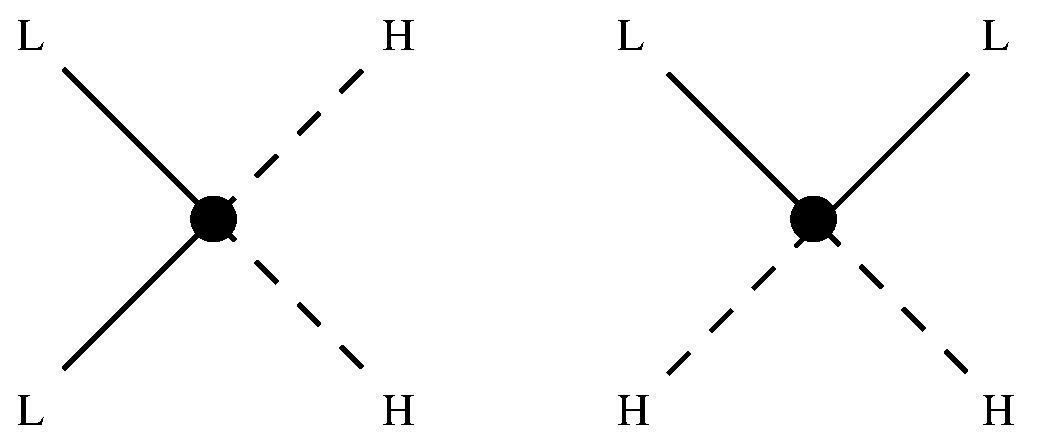
\includegraphics[width=9cm]{lflip.eps}
\caption{L-flipping processes generated by the effective vertex \eqref{L_eff}.}
\label{lflip_fig}
\end{figure}
There are two types of interactions induced by the effective
Lepton-Higgs vertex, 
%with $\Delta L =1$ and $\Delta L=2$, 
shown in  Fig.~\ref{lflip_fig}.
They generate the following processes relevant for leptogenesis:
\begin{align}
\notag
	L~~+~~L ~~\longleftrightarrow~~ H~~+~~H~  \\
\notag
	L~~+~~H ~~\longleftrightarrow~~ \ov{L}~~+~~H~,
\end{align}
%together with their inverse processes, and 
with the same set of processes
for antileptons.
However, since the relevant part of the $CPT$-odd interactions is time reversal invariant, 
the amplitudes for
direct and inverse processes are equal, and we therefore have 
only three different amplitudes, which we call  
$ A_{LL} $, $ A_{\ov{LL}} $ and $ A_{LH} $.
Denoting the corresponding reaction rates (per unit volume) by
$ W_{LL} $, $ W_{\ov{LL}} $, $ W_{L\ov{H}} $ and $ \ov{W}_{L\ov{H}} $,
where 
\begin{align*}
% first line
	W_{LL}   ~~=~~  &
		\int d\pi_p d\pi_q d\pi_k d\pi_r ~
		(2\pi)^4~ \delta^4 ( p + q - k - r )\,
		| A_{LL} |^2\, f_L^\eq(p)\, f_L^\eq(q)~, \\
% second line
	W_{\ov{LL}}   ~~=~~  &
		\int d\pi_p d\pi_q d\pi_k d\pi_r ~
		(2\pi)^4~ \delta^4 ( p + q - k - r )\,
		| A_{L\ov{H}} |^2\, f_L^\eq(p)\, f_{\ov{H}}^\eq(q)~, \\
% third line
	W_{LH}  ~~=~~  &
		\int d\pi_p d\pi_q d\pi_k d\pi_r ~
		(2\pi)^4~ \delta^4 ( p + q - k - r )\,
		| A_{L\ov{H}} |^2\, f_{\ov{L}}^\eq(p)\, f_H^\eq(q)~, \\
% fourth line
	\ov{W}_{LH}  ~~=~~  &
		\int d\pi_p d\pi_q d\pi_k d\pi_r ~
		(2\pi)^4~ \delta^4 ( p + q - k - r )\,
		| A_{LL} |^2\, f_{\ov{L}}^\eq(p)\, f_{\ov{L}}^\eq(q)~
\end{align*}
	(here $ f_{L,H}^\eq(p) $ are equilibrium distribution functions for Higgs
	and leptons),
	we can write the Boltzmann equations for the lepton number density as
\begin{equation}
\label{lepton_sys}
%\left\{~~
\begin{split}
% first line
	\lgr \p_t ~+~ 3H \rgr 
		n_L ~~=~~ &
	-\, 2\, W_{LL} \lgr \frac{n_L^2}{(n_L^\eq)^2} ~-~ 1 \rgr
	~~-~~
	W_{L\ov{H}} \lgr \frac{n_L}{n_L^\eq} ~-~ 
			\frac{n_{\ov{L}}}{n_{\ov{L}}^\eq} \rgr  \\
% second line
	\lgr \p_t ~+~ 3H \rgr 
		n_{\ov{L}} ~~=~~ &
	-\, 2\, W_{\ov{LL}} \lgr 
		\frac{n_{\ov{L}}^2}{(n_{\ov{L}}^\eq)^2} ~-~ 1 \rgr
	~~-~~
	\ov{W}_{L\ov{H}} \lgr \frac{n_{\ov{L}}}{n_{\ov{L}}^\eq} ~-~ 
			\frac{n_L}{n_L^\eq} \rgr  \\
\end{split}
%\right.
%\right._{~.}
\end{equation}
	(the factor of two in the RHS here reflects the fact 
	that the LL processes change the number of leptons by two).
	An important thing to note is that even though we could have 
	modified the dispersion relations for the Higgs field, 
	its $CPT$-violating parameter would not enter the equations for the lepton number
	density.

	Strictly speaking, Eqs.~\eqref{lepton_sys} only describe the evolution
	of the weakly interating leptons. 
	Obviously, for the purpose of leptogenesis, the equations for the total
	lepton number, including right-handed particles, are needed.
	We argue, however, that since the Yukawa interactions turning left-handed
	and right-handed particles into each other are rapid, 
	one can generalize the system \eqref{lepton_sys} for the 
	evolution of the total lepton number density 
\begin{equation}
\label{n_L_total}
	n_L  ~~=~~ n_\ell ~+~ n_E~
\end{equation}
	(here $ n_\ell $ is the number density of the left-handed leptons),
	which has an effective $ CPT $-odd parameter 
\[
	\eta_L ~~=~~ \frac{ g_\ell \eta_\ell ~+~ g_E \eta_E } { g_\ell ~+~ g_E }~.
\]

	As already mentioned,
	one also has to deal with the sphaleron processes, which change
	both baryon and lepton number densities.
	The general effect of sphalerons is to partly wash-out $ B + L $,
	while keeping $ B - L $ intact.
	Therefore, the system \eqref{lepton_sys} has to be completed with
	the equations for baryons.
	For our purposes it will be sufficient to use the linear
	temperature dependence approximation of the sphaleron rate
\cite{Kuzmin:1985mm,Khlebnikov:1988sr}. 
	The sphaleron contribution to the Boltzmann equation
	for $ n_L $, $ n_B $ is 
\cite{Kuzmin:1985mm,Moore:2000mx,Moore:2000ar}:
\begin{equation}
\label{sph_corr}
	\p_t\, (n_B + n_L)
	~~~=~~~ -\, \Gsph 
		\lgr   n_B - n_B^\eq \;~+~\;
		       n_L - n_L^\eq 
		\rgr~,
\end{equation}
	where
\[
	\Gsph ~~\simeq~~ \omega\, T~, \qquad\qquad 
	{\rm ~with~}
	\omega ~\simeq~ \,10^{-5}~.
\]
	Here, similarly to \eqref{n_L_total}, $ n_B $ is the total baryon number density
	$ n_B = \frac{1}{3}(n_Q + n_U + n_D) $, with a $ CPT $-odd parameter
\[
	\eta_B ~~=~~ \frac{g_Q \eta_Q ~+~ g_U \eta_U ~+~ g_D \eta_D} 
			    {g_Q ~+~ g_U ~+~ g_D}~,
\]
	and effectively the equilibrium distribution for baryons has 
	$ g_B \,\equiv\, \frac{1}{3}(g_Q + g_U + g_D) $.
	
	Next we make a well-justified assumption of 
	smallness of the chemical potentials,
\[
	\frac{n_i}{n_i^\eq} ~~=~~ e^{\mu_i/T} ~~\simeq~~ 1 ~~+~~ \mu_i/T~,
\]
	which enables us now to linearize the equations in $ \mu_i $.	
	The kinetic equations for $ n_L $ now look as
\begin{equation}
\label{kinetic_eqn_prelim}
\begin{split}
% first line
	\lgr \p_t ~+~ 3H \rgr
		n_L ~~=~~ & 
	-\, \lgr 4\, W_{LL} ~+~ 2\, W_{L\ov{H}} \rgr  \mu_L/T 
	~~-~~
	\omega\, T \lgr \mu_L/T ~+~ \mu_B/T \rgr 
	\\
% second line
	\lgr \p_t ~+~ 3H \rgr
		n_{\ov{L}} ~~=~~ &
	\phantom{-\,}
	\lgr 4\, W_{\ov{LL}} ~+~ 2\, \ov{W}_{L\ov{H}} \rgr  \mu_L/T 
	~~+~~
	\omega\, T \lgr \mu_L/T ~+~ \mu_B/T \rgr ~.
\end{split}
\end{equation}
	For the (anti)baryons the kinetic equations are the same except
	that there are no contributions from the lepton number violating
	rates. 
%	For the matter of generality, we assume that the dispersion
%	relations for baryons include $ CPT $-odd shifts as well.

	There are two possible sources for $CPT$-odd contributions 
	to the reaction rates: modified dispersion relations and 
	$CPT$-odd modifications of thermal rates. Now we observe that due to smallness of the chemical potential
	any $CPT$-odd effects in the reaction rates in the RHS of 
	\eqref{kinetic_eqn_prelim} can be neglected, as
	they induce effects of the 2nd order in the $CPT$-violating parameter, so that
	%As we argued, one can neglect both of them, and take
%	In our case, neither of them contribute, so we can take
	$ W_{\ov{LL}} = W_{LL} $ and
	$ \ov{W}_{L\ov{H}} = W_{L\ov{H}} $.

	From the above equations we only need their difference, the actual
	lepton (baryon) asymmetry.
	For convenience, we express the equilibrium number density in terms
	of the unmodified number density 
	$ n_i^0 = g_i/\pi^2 \cdot T^3 $
\[
	n_{i,\ov{i}}^\eq ~~=~~ n_i^0\, \left(\, 1 ~\mp~ 6\,\eta_i T \,\right)~,
	\qquad\qquad{i ~=~ L, B}~.
\]
%	where $ \theta_L = -6\, \eta_L $.
	The asymmetries $ Y_i $ then can be defined as
\[
	n_i ~~-~~ n_{\ov{i}} ~~\equiv~~ 2\, n_i^0 \cdot Y_i~,
	\qquad\quad Y_i ~~=~~ \mu_i/T ~~-~~ 6\,\eta_i T~.
\]
	
	We also introduce a dimensionless parameter $ \gamma $, 
	by extracting the explicit dependence on the temperature from
	the rate of L-processes:
%\begin{align*}
%% first line
%&	 n_L^0 ~~=~~   \delta \cdot T^3~, \\
%% second line
%&	H     ~~=~~   \frac{T^2}{2\, \alpha\, \Mpl}~, \\
% third line
%&	4\, W_{LL} ~~+~~ W_{L\ov{H}} ~~=~~ 
%		 \gamma\, \frac{T^6}{M_R^2}~, \\
%% fourth line
%&	\lambda ~~\equiv~~  \frac{2\,\alpha\,\gamma}{\delta} ~.
%\end{align*}
\begin{equation*}
	4\, W_{LL} ~~+~~ 2\, W_{L\ov{H}} ~~=~~ 
		 \gamma\, \frac{T^6}{M_R^2}~.
\end{equation*}
%	The explicit values of the above constants are
%	$ \alpha  ~=~ 0.3\, g_*^{-1/2} $ and 
%	$ \delta  ~=~ g_L/\pi^2 $.
%\begin{align*}
%% first line
%	\alpha & ~~=~~ 0.3\, g_*^{-1/2}~, \\
%% third line
%	\delta & ~~=~~ \frac{g_L}{\pi^2}~.
%\end{align*}
	The value of $ \gamma $ is determined by the explicit 
	cross-sections of the lepton-number flipping processes
	(see Fig.~\ref{lflip_fig}):
\begin{equation}
\label{gamma}
%	\gamma  ~~=~~ \frac{3}{2\pi^2}\, (N_g)^2\, |Y|^4~, 
	\gamma  ~~=~~ \frac{3}{2\pi^2}\, \lgr \sum |h_a|^2 \rgr^2~.
\end{equation}
%	where $ N_g = 3 $ is the number of generations of leptons.

	Now equations \eqref{kinetic_eqn_prelim} expressed in terms of
	$ Y_i $ read as:
\begin{equation}
\label{eqn_Y}
\left\{~~
\begin{split}
% first line
	g_L Y_L' 
	& ~~\;=~~\;
	\frac{0.6}{g_*^{1/2}}\, 
	\frac{\omega\,\Mpl}{T^2}\,
	\lgr g_L (\,Y_L~+~6\,\eta_L\,T\,) ~~+~~ 
	     g_B (\,Y_B~+~6\,\eta_B\,T\,)  \rgr 
	\;~~+
	\\
% second line
	& \;~~+~~\;  
	\frac{0.6\,\pi^2}{g_*^{1/2}}\, 
	\frac{\gamma\,\Mpl}{M_R^2}\,
	\cdot (\, Y_L ~+~ 6\,\eta_L\,T\,)\\
% third line
	g_B Y_B' 
	& ~~\;=~~\;
	\frac{0.6}{g_*^{1/2}}\, 
	\frac{\omega\,\Mpl}{T^2}\,
	\lgr g_L (\,Y_L~+~6\,\eta_L\,T\,) ~~+~~ 
	     g_B (\,Y_B~+~6\,\eta_B\,T\,)  \rgr 
	~~,
\end{split}
\right.
\end{equation}
	where the prime denotes differentiation with respect to
	the temperature.
	The quantity of the ultimate interest is the baryon asymmetry 
	at the present time (normalized, e.g. on the photon number density,
	$ n_\gamma = s / 7.04 $ \cite{Kolb:1990vq}). 
	Using $ Y_B $ to find the baryon asymmetry normalized on the entropy
	density $ s = \frac{2\pi^2}{45} g_* T^3 $, one can express the desired
	quantity as
\begin{equation}
\label{def_asy}
	\mathfrak{a}_B ~~=~~ 7.04\, \frac{45}{\pi^4}\, \frac{g_B}{g_*}\, Y_B
	~~\simeq~~ 0.6 \, Y_B 
		~~\equiv~~ (\, 6.1 ~\pm~ 0.3 \,)\times 10^{-10}~.
\end{equation}

	Note, that in the limit when the rate of sphaleron processes
	is very small, $ \Gsph \ll \Gamma_L $ ($ \Gamma_L $ is the rate
	of L-violating processes), one can solve the kinetic equations
	exactly. 
	In equation \eqref{eqn_Y} taking this is equivalent to 
	putting $ \omega $ to $ 0 $.
	Then the baryon asymmetry decouples and one has a simple 
	kinetic equation for $ Y_L $:
%	Then the kinetic equation takes the simple form
\begin{equation}
\label{btz_simple}
	Y_L' ~~=~~ \frac{\lambda\,\Mpl}{M_R^2} \,
			\lgr Y_L ~+~ 6\,\eta_L\, T \rgr~.
\end{equation}
	where we have introduced
\[
	\lambda ~~=~~ \frac{0.6\, \pi^2}
    		         {g_*^{1/2}\, g_L}\,\gamma~.
\]
	
	The general solution for \eqref{btz_simple} is
\[
	Y_L^{(\rm g)} ~~=~~ -\,\frac{6\,\eta_L\,M_R^2}{\lambda\,\Mpl}
		~-~ 6\eta_L\,T ~+~
		A\cdot e^{\frac{\lambda\, \Mpl}{M_R^2}\, T}~,
\]
	with an arbitrary constant $ A $.
	Requiring $ Y_L $ to stay close to its equilibrium value 
	$ - 6\eta_L T $ at high temperatures one has to 
% presume that 
	put $ A = 0 $:
\begin{equation}
\label{btz_sol_simple}
	Y_L ~~=~~ -\,6\,\frac{\eta_L\,M_R^2}{\lambda\,\Mpl}
		~-~ 6\eta_L\,T ~.
\end{equation}
%	(one might worry why we have been able to obtain a special
%	solution of equation \eqref{btz_simple} without essentially giving it
%	any input data; note, however, that in the sense of leptogenesis
%	the solution \eqref{btz_sol_simple} still has an arbitrary
%	constant $ M_R $ which has to be fixed).
	Now, Eq.~\eqref{btz_sol_simple} provides us with the freeze-out
	temperature
\begin{equation}
\label{T_R}
	T_R ~~\sim~~ \frac{M_R^2}{\lambda\,\Mpl}~,
\end{equation}
	as well as with an expression for the lepton asymmetry,
\begin{equation}
\label{Y_L_simple}
	Y_L^{\rm fr} ~~=~~ -\, 6\,\frac{\eta_L\,M_R^2}{\lambda\,\Mpl}~.
\end{equation}
	%Temperature $ T_R $ is the one at which the Hubble rate equals 
	%the L-process rate, as it was expected (see Section~\ref{intro}).
%	This is of course the temperature at which the Hubble rate equals 
%	the L-process rate.
%	We emphasize that \eqref{Y_L_simple} is only an estimate, 
%	and one needs a more careful numerical analysis for the final
%	result.
%	In any case, it is not $ Y_L $ that is of interest, but, rather,
%	the corresponding baryon asymmetry $ Y_B $.
	In accord with the standard leptogenesis, sphalerons diffuse
	half of the lepton number yield into the baryon number
\cite{Kuzmin:1985mm}, 
	thus also rendering one half of the quantity on the right hand side
	of Eq.~\eqref{Y_L_simple} an estimate for the BAU.
	
	This answer, however, was obtained under the assumption that
	the sphaleron rate was much less than the rate of 
	neutrino-mediated processes during the epoch of leptogenesis.
	In general, one notices that  there can be three different scenarios, 
	depending on the relative magnitudes of $ T_R $ and $ \Tsph $, the 
	temperature at which sphaleron processes become rapid.
	The first case, when $ T_R \gg \Tsph $ has just been discussed
	and the answer given by \eqref{Y_L_simple}.
	{\bf *** I stopped editing here}

%	One then is faced with three possible developments of the scenario.
%	The first one appears if $ \Tsph $, the temperature at which
%	sphaleron processes become rapid, is considerably lower than $ T_R $.
%%	As is well-known, the sphalerons turn half of the lepton number
%%	into baryon number.
%	In this case, during the leptogenesis epoch, 
%	i.e. at $ M_R > T > T_R $,
%	the sphalerons were very slow and could essentially be dropped 
%	from consideration,
%	thus leaving one with \eqref{Y_L_simple} as the lepton number yield.
%	Below $ T_R $, the lepton number stayed constant, as the 
%	lepton-flipping processes were too slow to keep equilibrium.
%	And, finally, at $ \Tsph $, the sphalerons kicked in and diffused
%	half of the lepton number \eqref{Y_L_simple} into the baryon number.

	The second possibility arises if the sphaleron epoch partially
	overlaps the leptogenesis epoch, i.e. if $ \Tsph \gtrsim T_R $.
	Strictly speaking, it is not quite correct to give direct
	estimates for this case, as the expression \eqref{T_R} for $ T_R $
	was derived under an assumption that sphalerons decouple.
	It is clear, however, that one can still use \eqref{T_R} for
	qualitative estimates, since it gives the temperature at which
	the rate of L-processes became slower than the Hubble rate.
	If $ \Tsph $ happens to be enough greater than $ T_R $, there
	existed a period during which both processes were in equilibrium.
%	[{\it
%	Qualitatively, one can estimate the resulting BAU as follows.
%	Fast lepton-switching processes kept the lepton number around
%	its equilibrium, while sphalerons brought the baryon number to
%	the same level.
%	Indeed, sphalerons do not change $ B - L $. 
%	Since heavy-neutrino-mediated processes changed $ L $ 
%	(and did not touch $ B $), the sphalerons had to adjust $ B $ 
%	accordingly. 
%	At temperature $ T_R $, the ``leptogenesis'' stopped, 
%	the lepton number froze at the level estimated by \eqref{Y_L_simple},
%	and the BAU must have been of the same level. 
%	}]
	To estimate the resulting BAU it is easier to switch to the
	basis of $ B + L $ - and $ B - L $ -violating operators.
	In this language, L-processes generate both  $ B + L $ and $ B - L $:
\[
	Y_{B-L} ~\simeq~ \frac 12 (\eta_B - \eta_L ) \cdot T_R~,\qquad
	Y_{B+L} ~\simeq~ \frac 12 (\eta_B + \eta_L ) \cdot T_R~.
\]	
	Sphalerons then wash out $ Y_{B+L} $, yielding the BAU to be
	$ \frac 12 (\eta_B - \eta_L ) \cdot T_R $.
	Note that $ \eta_L $ gives the same contribution here as in the 
	first case.
	Opposite to $ \eta_B $, which did not contribute in the first case
	due to the absence of B-flipping processes.
	
	The third case corresponds to $ \Tsph \approx T_R $.
	Then there was no epoch during which both processes
	were in equilibrium, and in this sense this case is more complicated.
	However, to get an estimate, the reasoning can be 
	the same.
	Whatever $ B $ and $ L $ at $ T = \Tsph $ were, the resulting
	lepton and baryon asymmetry after the sphaleron epoch only
	depended on the input $ B - L $.
	Of course, since L-processes only changed the lepton number,
	this $ B - L $ at  $ T \sim \Tsph \approx T_R $ can 
	again be estimated by \eqref{Y_L_simple}.
	It is clear, however, that this argument is rather crude and 
	one needs a more direct numerical analysis to obtain an actual
	number.

	To see which situation is more realistic, one needs an estimate
	for $ T_R $. 
	This temperature depends on $ M_R $ and, through \eqref{gamma},
	on the Yukawa couplings for heavy neutrinos, which together 
	combine into the Dirac masses of the light neutrinos:
\begin{equation}
\label{T_R_eff}
	T_R  ~~\propto~~ \frac{M_R^2}{\Mpl \lgr \sum |h_a|^2 \rgr^2}
		~~\equiv~~ \frac{v^4}{\Mpl (\meff)^2}~,
\end{equation}
	where we have introduced an ``effective'' neutrino mass
\[
	\meff ~~=~~ \sum m_{\nu_a} ~~=~~ \frac{\sum |h_a|^2}{M_R}\,v^2~.
\]
	The biggest contribution to the asymmetry is expected in the case
	when the L-processes freeze out early. 
	Note that the denominator in \eqref{T_R_eff} is dominated by the mass
	of the heaviest neutrino.
	It is clear that in order to make $ T_R $  attain its minimal
	value one has to apply the biggest estimates on the neutrino masses.
	Thus one is interested in the highest of the lower limits on
	$ \meff $.
	In particular, $ \meff $ cannot be smaller then the atmospheric limit
	on the neutrino mass difference $ \sqrt{\Delta m_{\rm atm}^2}$:
\[
	\meff ~~>~~ \sqrt{\Delta m_{\rm atm}^2} ~~\simeq~~ 0.05~\eV~.
\]
	To get a lower limit on $ T_R $, one can use the cosmological
	bound on the sum of neutrino masses
\[
	\sum m_{\nu_a} ~~\leq~~ 0.65~\eV~.
\]
	These bounds translate into the range of realistic values for the
	freeze-out temperature:
\[
	10^{12}~\GeV ~~<~~ T_R ~~<~~ 10^{14}~\GeV~.
\]
	One now can compare these typical values of $ T_R $ with the 
	sphaleron ignition temperature $ \Tsph $, which is estimated
	to be of the order $ 10^{12}~\GeV $ 
\cite{Buchmuller:2005eh}.
	As the freeze-out temperature appears to be slightly greater
	than $ \Tsph $ and 	
	it is most likely then, that there was no period when
	both sphalerons and L-processes were active, but at the same
	time, there was no significant separation between the characteristic 
	temperatures of their activity.
	That means that neither of the processes can be neglected,
	and corresponds to the third scenario introduced above.

	To solve the system of kinetic equations, one also has to 
	add proper initial conditions.
	It is reasonable to impose these initial conditions at the temperatures
	where the essential part of leptogenesis begins, which we
	take to be $ M_R = 10^{15}~\GeV $.
	At that time, leptons were in their equilibrium, which
	had a nonzero value of the lepton number defined by $ \eta_L $.
	As we have seen, this hypothesis is quite sensible since 
	the freeze-out temperature $ T_R $ is sufficiently smaller than
	$ M_R $.
	Even if one starts off out of equilibrium, the fast L-processes
	will quickly bring the system back into it.
	Consequently, if we take the initial leptogenesis temperature
	to be some $ T ~=~ M ~>~ M_R $, then at $ T~=~M_R $ one would
	still have equilibrium in the lepton sector, so the above
	choice of the leptogenesis temperature is quite justified.

	As for baryons, we are less legitimate to assume them to be in
	equilibrium, since at those times there were no baryon number
	violating processes to maintain it.
	Theoretically their initial asymmetry could have been arbitrary,
	but aesthetically it is more natural to assume it zero
	(otherwise the whole problem of obtaining a non-zero BAU would
	not be much contented):
\begin{align*}
	Y_L\bigl|_{M_R} & ~~=~~ \theta_L\, M_R~, \\
	Y_B\bigl|_{M_R} & ~~=~~ 0~.
\end{align*}
	

%\subsection{Account for the sphaleron rate}
%
%	We now turn to Eq.\eqref{T_R}, which determines the time when
%	the lepton-flipping processes became slower than the Hubble
%	rate.
%	To get an upper limit on $ T_R $, one can use the atmospheric
%	limit on neutrino masses, $ m_\nu^i > 0.05~\eV $ 
%	to estimate the ratio $ M_R^2 / Y^4 $.
%	For $ M_R \sim 10^{15}~\GeV $ one obtains temperature $ T_R^{max} $ 
%	of the order $ 10^{13}~\GeV $.
%	To get a lower limit on $ T_R $, one can use the cosmological
%	bound on total neutrino masses
%\[
%	\sum (m_i)^2 ~~\leq~~ (0.65~\eV)^2~,
%\]
%	which yields $ T_R^{min} $ of the order of $ 10^{11}~\GeV $. 
%	It is estimated that $ \Tsph \sim 10^{12}~\GeV $ [ref]. 
%	One can see that typical values of parameters at best 
%	lead to $ T_R $ being slightly greater than $ \Tsph $.
%	It is most likely then, that there was no period when
%	both sphalerons and L-processes were active, but at the same
%	time, there was no separation between the characteristic 
%	temperatures of their activity.
%	That means that neither of the processes can be neglected,
%	what corresponds to the third scenario introduced above.
%%	One can see that reasonable parameters yield the third scenario
%%	described above.
%	To obtain a quantified prediction for BAU one certainly needs
%	to consider carefully both sphaleron processes and L-processes
%	in the kinetic equations.
%
%	For our purposes it will be sufficient to use the linear
%	temperature dependence approximation of the sphaleron rate [ref]. 
%	The general effect of sphalerons is to partly wash-out $ B + L $,
%	while keeping $ B - L $ intact.
%	Schematically, the sphaleron contribution to the Boltzmann equation
%	for $ n_L $, $ n_B $ is [KRS,Moore]:
%\begin{equation}
%\label{sph_corr}
%	\frac{d}{dt}\, n_B~,~~
%	\frac{d}{dt}\, n_L
%	~~~\supset~~~ -\, \Gsph 
%		\lgr   n_B - n_B^\eq \;~+~\;
%		       n_L - n_L^\eq 
%		\rgr~,
%\end{equation}
%	where
%\[
%	\Gsph ~~\simeq~~ \omega\, T~, \qquad\qquad 
%	{\rm ~with~}
%	\omega ~\simeq~ \,10^{-5}~.
%\]
%%\[
%%	\Gsph ~~\simeq~~ \frac{39}{4}\,\omega T~, \qquad\qquad 
%%	{\rm ~with~}
%%	\omega ~~\simeq~~ \,10^{-6}~.
%%\]
%%	One then includes the account for the sphaleron rate \eqref{sph_corr}
%%	into the kinetic equations \eqref{kinetic_eqn_prelim}.
%%	Also, one has to add similar equations for the baryon density $ n_B $.
%%	Instead of working with the measures of asymmetry $ Y_L $ and 
%%	 $ Y_B $ it is technically more convenient to introduce the
%%	deviation from equilibrium $ \Upsilon_{L,B} $:
%%\[
%%	\Upsilon_i ~~=~~ Y_i ~-~ \theta_i T ~~=~~ \mu_i/T~,
%%	\qquad\qquad i~=~L,B~.
%%\]
%%	(now that we are tracking both lepton and baryon numbers 
%%	simultaneously, we have to explicitly indicate which quantites
%%	are related to which sector, and therefore we will be appending
%%	a subscript L or B where appropriate).
%%	In terms of $ \Upsilon_{L,B} $
%%	the kinetic equations can be written in a more symmetric way:
%
%	One then includes the account for the sphaleron rate \eqref{sph_corr}
%	into the kinetic equations \eqref{kinetic_eqn_prelim}:
%\begin{equation}
%\label{eqn_ups}
%\left\{~~
%\begin{split}
%% first line
%	g_L Y_L' 
%	& ~~\;=~~\;
%	\frac{0.6}{g_*^{1/2}}\, 
%	\frac{\omega\,\Mpl}{T^2}\,
%	\lgr g_L (\,Y_L~+~6\,\eta_L\,T\,) ~~+~~ 
%	     g_B (\,Y_B~+~6\,\eta_B\,T\,)  \rgr 
%	\;~~+
%	\\
%% second line
%	& \;~~+~~\;  
%	\frac{0.6}{g_*^{1/2}}\, 
%	\frac{\gamma\,\Mpl}{M_R^2}\,
%	\cdot (\, Y_L ~+~ 6\,\eta_L\,T\,)\\
%% third line
%	g_B Y_B' 
%	& ~~\;=~~\;
%	\frac{0.6}{g_*^{1/2}}\, 
%	\frac{\omega\,\Mpl}{T^2}\,
%	\lgr g_L (\,Y_L~+~6\,\eta_L\,T\,) ~~+~~ 
%	     g_B (\,Y_B~+~6\,\eta_B\,T\,)  \rgr 
%	~~.
%\end{split}
%\right.
%\end{equation}
%
%%\begin{equation}
%%\label{eqn_ups}
%%\left\{~~
%%\begin{split}
%%% first line
%%	\delta_L \lgr \Upsilon_L' ~~+~~ \theta_L \rgr
%%	& ~~\;=~~\;
%%	2\, \alpha\chi \Mpl \cdot T^{-2} 
%%	\lgr \delta_L \Upsilon_L ~~+~~ \delta_B \Upsilon_B \rgr 
%%	\;~~+~~\;
%%	2\, \alpha\gamma\, \frac{\Mpl}{M_R^2} \cdot \Upsilon_L \\
%%% second line
%%	\delta_B \lgr \Upsilon_B' ~~+~~ \theta_B \rgr
%%	& ~~\;=~~\;
%%	2\, \alpha\chi \Mpl \cdot T^{-2} 
%%	\lgr \delta_L \Upsilon_L ~~+~~ \delta_B \Upsilon_B \rgr 
%%	~~.
%%\end{split}
%%\right.
%%\end{equation}
%%	This is a purely technical simplification, since
%	The quantity of interest is the baryon asymmetry normalized on the
%	photon number density at the present time, which can be expressed
%	in terms of $ Y_B $,
%\begin{equation}
%\label{def_asy}
%	\mathfrak{a}_B ~~=~~ 7.04\, \frac{45}{\pi^4}\, \frac{g_B}{g_*}\, Y_B
%	~~\simeq~~ Y_B 
%		~~\equiv~~ (\, 6.1 ~\pm~ 0.3 \,)\times 10^{-10}~.
%\end{equation}
%
%	One now has to solve system \eqref{eqn_ups} numerically.
%	It is reasonable to impose initial condition at the temperatures
%	where the essential part of leptogenesis begins, which we
%	take to be $ M_R = 10^{15}~\GeV $.
%	At these temperatures, leptons were in their equilibrium, which
%	had a nonzero value of the lepton number defined by $ \eta_L $.
%	As we have seen, this hypothesis is quite sensible since 
%	the freeze-out temperature $ T_R $ is sufficiently smaller than
%	$ M_R $.
%	Even if we start off out of equilibrium, the fast L-processes
%	will quickly bring the system back into it.
%	Consequently, if we take the initial leptogenesis temperature
%	to be some $ T ~=~ M ~>~ M_R $, then at $ T~=~M_R $ one would
%	still have equilibrium in the lepton sector, so the above
%	choice of the leptogenesis temperature is quite justified.
%
%	As for baryons, we are less legitimate to assume them to be in
%	equilibrium, since at those times there were no baryon number
%	violating processes to maintain it.
%	Theoretically their initial asymmetry could have been arbitrary,
%	but aesthetically it is more natural to assume it zero
%	(otherwise the whole problem of obtaining a non-zero BAU would
%	not be much contented):
%\begin{align*}
%	Y_L\bigl|_{M_R} & ~~=~~ \theta_L\, M_R~, \\
%	Y_B\bigl|_{M_R} & ~~=~~ 0~.
%\end{align*}
		


%%%%%%%%%%%%%%%%%%%%%%%%%%%%%%%%%%%%%%%%%%%%%%%%%%%%%%%%%%%%%%%%%%%%%%
%%%%%%%%%%%%%%%%%%%%%%%%%%%%%%%%%%%%%%%%%%%%%%%%%%%%%%%%%%%%%%%%%%%%%%
%
%        BARYON ASYMMETRY OF THE UNIVERSE: SUPPLY AND DEMAND  
%
%%%%%%%%%%%%%%%%%%%%%%%%%%%%%%%%%%%%%%%%%%%%%%%%%%%%%%%%%%%%%%%%%%%%%%
%%%%%%%%%%%%%%%%%%%%%%%%%%%%%%%%%%%%%%%%%%%%%%%%%%%%%%%%%%%%%%%%%%%%%%
\section{Baryon Asymmetry of the Universe: ~Supply and Demand}

	We set up the problem inverse to the Cauchy problem:
%	given the present-time baryon abundance \eqref{def_asy},
	we set to find the values of $ \eta_L $ and $ \eta_B $ 
	big enough to generate the present-time baryon 
	abundance \eqref{def_asy}.
	Since equations \eqref{eqn_Y} are linear in $ Y_i $,
	it will be sufficient to consider two opposite cases
\[
	\eta_L ~~\neq~~ 0,\qquad\qquad \eta_B ~~=~~ 0~, 
\]
	and
\[
	\eta_L ~~=~~ 0,\qquad\qquad \eta_B ~~\neq~~ 0~.
\]
	Qualitative features of the solution of Eq.~\eqref{eqn_Y} can
	be inferred only in an assumption of small sphaleron rate,
	which unfortunately is only approximately true.
	The first case should be close to the scenario considered in
	Section~\ref{rates}  --- 
	leptons freeze out, and at lower temperatures get converted
	into baryons. 
	The resulting BAU thus should weakly depend on the sphaleron
	rate.
	For the second case, the sphaleron rate is more crucial, since
	only due to sphalerons the mutual lepto- and baryogenesis is
	made possible. 
	

%	We have fixed the parameter $ M_R $ of equations \eqref{eqn_ups},
%	as the result evidently is very weakly dependent on it:
%	provided that $ M_R \gg T_R $, the L-processes will quickly bring
%	leptons into equilibrium which will be maintained down to
%	$ T = T_R $.
	We have fixed the parameter $ M_R $ to be of the order of 
	$ 10^{15}~\GeV $.
	There is a parameter which is not strictly fixed,
	the ``effective'' neutrino mass $ \meff $, which enters
	through the
	L-processes rate $ \gamma $ (see Eq.~\eqref{gamma}),
	and which we allow to vary within the limits 
\[
	0.01~\eV ~~<~~ \meff ~~<~~1~\eV~.
%	0.05~\eV ~~<~~ \meff ~~<~~0.65~\eV~.
\]
	Fig.~\ref{b_dom_asymm_bau} shows the evolution of the baryon
	asymmetry function $ Y_B $ (see Eq.~\eqref{def_asy}) in the case
	$ \eta_b \neq 0 $, versus the equilibrium baryon asymmetry 
	$ Y_B^{\eq} $.
	Since one starts from zero asymmetry, function $ Y_B $ overshoots
	the equilibrium curve, and not even starting to follow it, freezes out
	at lower temperatures. 
\begin{figure}
\includegraphics[width=9cm,angle=270]{b_dom_asymm_bau.ps}
\caption{Baryon asymmetry function $ Y_B $ and equilibrium baryon asymmetry vs 
	temperature in the case of the LV in the baryon sector. 
	The parameter $ \eta_B $ was chosen such as to produce the observed BAU 
	\eqref{def_asy} at the freeze-out.}
\label{b_dom_asymm_bau}
\end{figure}

	Similar picture for LV in the lepton-sector is shown 
	in Fig.~\ref{l_dom_asymm_bau}.
	The evolution starts from the equilibrium value of the (lepton)
	asymmetry, and, depending on the freeze-out temperature $ T_R $,
	$ Y_L $ follows the equilibrium curve for some time.
	Due to this tracking of the equilibrium, the contribution of $ \eta_L $ 
	to the final asymmetry is suppressed relative to the that produced by the same 
	absolute value of $ \eta_B $.
\begin{figure}
\includegraphics[width=9cm,angle=270]{l_dom_asymm_bau.ps}
\caption{
	Lepton asymmetry vs temperature in the case of the LV in the lepton sector.
	Similarly to Fig.~\ref{b_dom_asymm_bau}, the parameter $ \eta_L $ was fitted
	to yield the observed value of baryon asymmetry.
	Depending on $ \meff $, $ Y_L $ may follow the equilibrium for longer time.
	For convenience of perception, the plot is presented upside-down.
	}
\label{l_dom_asymm_bau}
\end{figure}

	In Figs.~\ref{b_dom_asymm_bau}, \ref{l_dom_asymm_bau}, the LV parameters were
	chosen such as to yield the observed BAU in the end. 
	In general, their values depend 
%on the freeze-out temperature, which in
%	its turn depends on 
	the effective neutrino mass $ \meff $.
	Fig.~\ref{scan_fig} exhibits this dependence for a phenomenologically
	viable range of $ \meff $, the most interesting region being that of
	the small mass.
	One notices that $ \eta_B $ does not change much in the ``physical'' region.
	For $ \eta_L $-scenario, in contrast, 
%	$ \meff $ defines the decoupling temperature
	$ \meff $ is defining in terms of the decoupling temperature
	and the production rate of asymmetry.
	Thus, in different regions of the plot on Fig.~\ref{scan_fig}, $ \eta_L $
	and $ \eta_B $ compete in production ``efficiency''.
	At large values of $ \meff $, the $ \eta_L $-generated asymmetry 
	(Fig.~\ref{l_dom_asymm_bau}) tracks the equilibrium curve for too long.
	The $ \eta_B $-generated asymmetry 
	(Fig.~\ref{b_dom_asymm_bau}), on the other hand, 
	always overshoots the equilibrium, and as a result $ \eta_L $ loses
	to $ \eta_B $ in efficiency.
	In contrast, at small $ \meff $, $ Y_L $ wins by decoupling early 
	from the ever-decreasing equilibrium value. 
	The $ \eta_B $-scenario in this case is much less efficient due to large
	freeze-out temperature $ T_R $.

	Concluding the numerical analysis, we note that, as it was easily foreseen, 
	although the required values of $ \eta_L $, $ \eta_B $ are quite
	small, they are still many orders of magnitude larger than
	current experimental bounds.
\begin{figure}
\includegraphics[width=9cm,angle=270]{scan_log.ps}
\caption{CPT-odd parameters $ \eta_L $, $ \eta_B $ necessary to generate
	the observed BAU versus the neutrino mass.
	The left vertical line indicates the atmospheric limit on $ m_\nu $,
	while the right vertical line shows the cosmological upper 
	bound on $ m_\nu $.}
\label{scan_fig}
\end{figure}
	This definitely excludes CPT-odd leptogenesis at the level of
	mass dimension five from applicability.

\subsection{Operators of dimension seven and higher}

	We can extend this assertion to theories with higher-dimensional 
	CPT-odd operators. 
	We do not repeat the analysis of the kinetic equation 
	for this case.
%	for the case of higher-dimensional operators.
	We note that within a couple of orders of magnitude, the resulting BAU
	is determined by the initial equilibrium lepton asymmetry
	at the freeze-out time, $ \theta_L\,T_R $ in the case considered
	above, see Fig.~\ref{b_dom_asymm_bau}.
	The presented analysis has only brought in more 
	detailed numerical answers, but it could not alter the fact that
	dimension five operators are incapable of carrying out successful
	baryogenesis.
	We expect the same to be true with the case of higher-dimensional
	operators, and therefore make an estimate of resulting BAU 
	via equilibrium asymmetry.


	For higher-dimensional operators, the relevant LV part of the 
	Lagrangian is
%	We can proceed iteratively, excluding higher-dimensional operators 
%	one by one.
%	Starting with dimension seven, the relevant LV part of the Lagrangian 
%	is
\[
	\mc{L} ~~=~~ \eta^{(7)}_{\kappa\lambda\mu\nu\rho}\,
	\ov{\psi} \gamma^\kappa \md^\lambda \md^\mu \md^\nu \md^\rho \psi
	~~+~~ ...\,.
\]
	An operator $ \eta^{(n)} $ of mass dimension $ n $ makes a CPT-odd contribution to
	the dispersion relations:
\begin{equation}
\label{disp_rel_n}
	E ~~=~~ p ~+~ \frac 12 m^2/p ~+~ \frac 12 \eta^{(n)} p^{n-3}~,
\end{equation}
	which, in their turn shift the equilibrium number density:
\[
	n_B^\eq ~~=~~ n_B^0 \cdot \left(\, 1 ~-~ \frac{(n-1)!}{4} \eta^{(n)} T^{n-4}
					\,\right)~.
\]
	This allows us to find the freeze-out value of the baryon asymmetry:
\begin{equation}
\label{Y_B_n}
	Y_B ~~\sim~~ -\, \frac{(n-1)!}{4} \, \eta^{(n)} \,T^{n-4}_R~.
\end{equation}
	
	Observational bound on $ \eta^{(n)} $ can be obtained by a generalizations
	of the Gagnon and Moore bounds 
\cite{Gagnon:2004xh} 
	on CPT-odd interactions.
	If there is a CPT-odd operator in the lepton sector, it will modify dispersion
	relations for the electron according to \eqref{disp_rel_n}.
	Therefore, the ultra-high energy cosmic rays would be kinematically allowed to 
	emit positron-electron pairs, and therefore not be observed.
	Existence of rays with energy about $ \Eray ~\sim~ 3\times10^{11}~\GeV $ then 
	puts a limit on $ \eta^{(n)} $:
\begin{equation}
\label{bound_eta_n}
	\eta^{(n)} ~~<~~ 
	2^{n-3} \frac{m_p^2}{\Eray^{n-2}}~(\GeV)^{(4-n)}~.
\end{equation}
%	Such bounds will, however, be directly applicable only to higher-dimensional operators
%	of the photon sector.
%	If there is a CPT-odd operator $ \xi^{(n)}_{\kappa\lambda\mu...} $ in the 
%	photon sector, it will modify dispersion relations of the photon similarly
%	to \eqref{disp_rel_n}, where the modification will have different signs
%	for photons of opposite polarizations.
%	Ultra-high energy cosmic rays would then be kinematically allowed to
%	emit photons and lose energy, and therefore not be observed.
%	Existence of rays with energy about $ \Lray ~\sim~ 3\times10^{11}~\GeV $ then 
%	puts a limit on $ \xi^{(n)} $:
%\begin{equation}
%\label{bound_xi_n}
%	\xi^{(n)} ~~<~~ 
%	2\, \left( \frac{m_p}{\Lray} \right)^2\, \left(\frac{2}{\Lray}\right)^{n-4}
%	~~=~~
%	\frac{2}{9}\, 10^{-22}\cdot 10^{-11(n-4)}~(\GeV)^{(4-n)}~.
%\end{equation}
%	We speculate that this limit, modulo loop factor, can be transferred on the 
%	fermionic sector, by arguing that the existence of  non-zero $ \xi^{(n)} $ 
%	should generate non-zero operator $ \eta^{(n)} $, which, in the absence of fine-tuning, 
%	should respect the same bound.
%
	Substituting \eqref{bound_eta_n} into \eqref{Y_B_n} and then into 
	\eqref{def_asy} one then obtains
%\begin{align}
%\notag
%	\mathfrak{a}_B ~~<~~ 5 \times 10^{-22}\cdot \left [ \frac{T_R}{10^{11}~\GeV} 
%							\right ]^{n-4}~.
%	\\
%\notag
%	\text{\it Or is it better to have $\Eray$ instead of explicit numbers?}
%\end{align}
\begin{align}
\notag
	\mathfrak{a}_B ~~\simeq~~ 0.6 \, Y_B
	~~<~~ 
		0.6 \times 2^{n-5} (n\,-\,1)!\, \frac{m_p^2\, T_R^{n-4}}{\Eray^{n-2}}~.
\end{align}

	The condition that this asymmetry should reach the observed value then translates
	into
\[
	n~~>~~X~.
\]
	Therefore, successful baryogenesis is only possible in the presence of LV operators
	starting from dimension XX, which of course is rather 
% awkward and 
	unnatural to assume.


%%%%%%%%%%%%%%%%%%%%%%%%%%%%%%%%%%%%%%%%%%%%%%%%%%%%%%%%%%%%%%%%%%%%%%
%%%%%%%%%%%%%%%%%%%%%%%%%%%%%%%%%%%%%%%%%%%%%%%%%%%%%%%%%%%%%%%%%%%%%%
%
%                            DISCUSSION
%
%%%%%%%%%%%%%%%%%%%%%%%%%%%%%%%%%%%%%%%%%%%%%%%%%%%%%%%%%%%%%%%%%%%%%%
%%%%%%%%%%%%%%%%%%%%%%%%%%%%%%%%%%%%%%%%%%%%%%%%%%%%%%%%%%%%%%%%%%%%%%
\section{Discussion}

	We have seen that the presence of CPT-odd interactions is theoretically capable
	of replacing \emph{two} of Sakharov's conditions of baryogenesis: non-conservation 
	of CP symmetry and absence of thermodynamical equilibrium.
	The reason for this is that non-zero lepton (or baryon) asymmetry is already present 
	in the state of equilibrium
\cite{Dolgov:1981hv}.
	It is of course aesthetically more correct to consider LV interactions in the 
	lepton sector,
	since otherwise the presence of equilibrium baryon asymmetry would render the 
	problem too trivial.
	We, however, have considered both possibilities, owing to  simplicity of the kinetic
	equations.
	Another attracting property is that CPT-odd leptogenesis does not require more than
	one heavy neutrino, whereas conventional leptogenesis requires more than one flavor
	of majorana neutrinos.

	One important feature that we have found is that, to the linear order in CPT-odd 
	parameters, LV interactions that do not modify the dispersion relations effectively 
	drop out of the leptogenesis process.
	A brief explanation for this is that one necessary needs a shift of energies
	in the equilibrium for particles and antiparticles, which is provided by the 
	interactions which do modify the dispersion relations. 
	Other types of interactions, such as $ a^\mu\, \ov{L}H \md_\mu e_R $,
	can only manifest themselves in the kinetic equations where their contribution
	is always additionally suppressed 
	(see discussion after Eq.\eqref{kinetic_eqn_prelim}).
	At earlier times, there could have been interactions which possibly could 
	shift the balance between heavy neutrinos and antineutrinos, such as 
\begin{equation}
\label{heavy_LV_oper}
	\mathcal{L}_{LV} ~~\supset~~
	 b^\mu \ov{L} H \md_\mu \ov{N} \qquad\qquad \text{[in terms of Weyl fermions]}
\end{equation}
	However, below $ T ~=~ M_R $ all these effects
	were already washed-out by the stronger equilibrium processes.
	The effective remnants of \eqref{heavy_LV_oper}, $ \ov{L}H \md_\mu H \ov{L} $, 
	were additionally suppressed by $ M_R $ compared to the primary L-flipping processes
	(see Fig.~\ref{lflip_fig}).
	
	An approximate magnitude of the lepton asymmetry can be estimated by calculating
	the equilibrium asymmetry at the freeze-out temperature (the one at which the
	Hubble rate exceeds the rate of L-processes)
\cite{Bertolami:1996cq}.
	We have observed that the freeze-out temperature of the lepton asymmetry is
	estimated to be very close to the epoch of sphaleron activity.
	Thus, to obtain a more detailed answer, one should solve the corresponding 
	Boltzmann equations involving the sphaleron rate.

	It is no wonder that the current limits on LV interactions (in particular on those,
	which modify the dispersion relations), exclude virtually any scenario of successful
	CPT-odd leptogenesis.
	In fact, these limits are so strong, that this verdict can also be extended to 
	higher-dimensional LV operators.
	Arguments analogous to those of Gagnon and Moore
\cite{Gagnon:2004xh} 
	allow one to exclude CPT-odd
	leptogenesis due to operators up to mass dimension nine.
	This already sounds convincing enough that, although equilibrium leptogenesis
	due to Lorentz violation is theoretically viable, phenomenologically it appears
	to be impossible.


\bibliographystyle{apsrev}
\bibliography{genesis}

\end{document}
